\documentclass[10pt,letterpaper]{article}
\usepackage[preprint]{tmlr}

\input{math_commands.tex}
\usepackage{amsmath}
\usepackage{booktabs}
\usepackage{tabularx}
\usepackage{array}
\usepackage{graphicx}
\usepackage{float}
\usepackage{hyperref}
\usepackage{url}
\usepackage{xcolor}
\usepackage{tikz}
\usetikzlibrary{arrows.meta,calc,positioning}

\newcolumntype{Y}{>{\raggedright\arraybackslash}X}
\newcommand{\cov}{\mathrm{Cov}}
\newcommand{\pTen}{\mathrm{P10}}
\definecolor{plannerblue}{RGB}{43,95,151}
\definecolor{learnedorange}{RGB}{214,121,42}
\definecolor{memorygreen}{RGB}{71,129,92}
\definecolor{oraclegray}{RGB}{112,112,112}

\title{Towards Affordance in Robotics Application:\\[0.35em]
Model-Based vs.\ Non-Model-Based Approaches\\[0.45em]
\large Learning Against an Explicit Frontier Planner Under Partial Observation}

\author{\name Student: Kanan Gurbanli \\
\addr Student Number: 25218029 \\
\addr MSc Integrated Machine Learning Systems \\
\addr Department of Electronic and Electrical Engineering \\
\addr University College London \\
\addr GitHub repository: \href{https://github.com/Kanuxa/Gridworld-main}{github.com/Kanuxa/Gridworld-main}
\AND
\name Supervisor: Dr.\ Yu Wu \\
\addr Department of Electronic and Electrical Engineering \\
\addr University College London
}

\def\month{08}
\def\year{2026}
\def\openreview{}
\setlength\aftertitskip{0.12in plus 0.1in minus 0.08in}

\begin{document}
\raggedbottom

\fancyhead[L]{\small ELEC0054: Research Project 25/26 - Final Report}
\fancyhead[R]{}
\fancypagestyle{plain}{%
  \fancyhf{}
  \fancyhead[L]{\small ELEC0054: Research Project 25/26 - Final Report}
  \fancyhead[R]{}
  \fancyfoot[C]{\thepage}
  \renewcommand{\headrulewidth}{0.4pt}}
\fancypagestyle{empty}{%
  \fancyhf{}
  \fancyhead[L]{\small ELEC0054: Research Project 25/26 - Final Report}
  \fancyhead[R]{}
  \fancyfoot[C]{\thepage}
  \renewcommand{\headrulewidth}{0.4pt}}
\maketitle
\vspace{-0.30in}

\begin{abstract}
This study examines whether learned decision mechanisms improve safe exploration for autonomous robotic inspection or search in a partially known, hazard-prone site. The supplied Gridworld and initial deterministic sweep baseline establish the shared task; the work develops and evaluates controllers, not a robotics simulator. Every deployable controller receives the same 5x5 egocentric observation and may construct memory; a full-map oracle is reported separately and is not deployable. The project compares learned action and target-selection policies with a heading- and thermal-aware, partial-observation frontier planner developed from the supplied sweep. On a held-out, map-matched 50-episode 15x15 test, the planner records 71.41\% mean coverage and 67.96\% P10 coverage, above the selected spatial-target PPO checkpoint (67.32\%, 62.18\%) and planner-residual PPO checkpoint (68.80\%, 62.67\%). Their paired mean coverage differences relative to the planner are $-4.10$ percentage points (95\% bootstrap confidence interval [--5.67, --2.67]; $p=4.06\times10^{-5}$) and $-2.61$ points ([--3.98, --1.25]; $p=0.0038$), respectively. Two further map-matched sensitivity tests of the residual checkpoint---15\% visual-object dropout and a one-resource setting---are inconclusive (their intervals include zero). On 31x31 maps, archived single-seed summaries show the same numerical ordering (66.39\% versus 65.82\% mean; 64.20\% versus 63.89\% P10). The 15x15 inference concerns these fixed saved checkpoints across fresh maps, not a population of training seeds; each PPO configuration still has one completed training run.
\end{abstract}

\section{Introduction}

Robotic exploration requires more than moving toward an immediate reward. The motivating application is an autonomous mobile robot undertaking inspection or search in an incompletely mapped, potentially hazardous site: it must build a useful local map, avoid unsafe regions, conserve its operating budget, and select informative locations before it exhausts time or resources. These decisions affect mission coverage directly: unnecessary revisits consume time and energy, while unsafe routes can prevent the robot from reaching informative areas. This project studies that decision layer in a compact Gridworld designed around operational affordances. Objects can be harmful or restorative, temperature changes movement cost, and only a local egocentric observation is visible at any instant. In this abstraction, health and energy stand for safety and operating margins; they do not claim to model a particular robot platform, perception stack, or actuator. The Gridworld environment and its initial deterministic sweep baseline were supplied as the project starting point. The contribution is therefore controller development and an auditable comparison within that fixed environment, not the design of a robotics simulator. The task isolates a practical choice in exploration-system design: should the controller learn its decisions from experience, or should it use an explicit map and planning rules derived from the task? Existing learning and frontier-planning methods motivate both choices, but they do not answer this question under one shared observation boundary, metric, and map-generation protocol.

The project began as an attempt to solve the baseline 15x15 game with learned models. It evolved into a controlled two-sided investigation. In parallel with recurrent DQN, PPO with random network distillation (RND), and R2D2-style experiments, a simple deterministic controller was refined into map-based planning methods. The final partial-observation frontier planner recorded the highest deployable summary. This prompted two final learned experiments that retain the planner as a route executor or strategic prior. The selected saved PPO checkpoints and unchanged planner were then tested on a fresh, common set of 50 maps. Neither learned hybrid exceeded the planner on mean or P10 coverage in that held-out paired test. The environment was also enlarged to 31x31 as a descriptive single-seed check; the planner again recorded higher mean and P10 coverage there.

This report makes four contributions. First, starting from the supplied Gridworld and deterministic sweep, it preserves an auditable taxonomy of the learned and non-learned controller families rather than presenting only the highest observed summary. Second, it separates the shared-observation deployable conditions from a privileged full-information oracle. Third, it reports both mean coverage and a lower-tail metric, the tenth percentile (P10), because an exploration controller should be assessed beyond its average score. Fourth, it supplies a held-out paired 15x15 test of the final planner and two selected PPO checkpoints, while keeping the 31x31 and single-training-seed evidence explicitly descriptive.

The single research question is: \emph{under the shared partial-observation interface, can a learned controller---either standalone or planner-assisted---exceed the partial-observation frontier planner in mean and P10 coverage?} The remainder of the report positions that question in the literature, specifies the common evaluation boundary, reports the measurements, and then interprets their scope.

\section{Related work}

\subsection{Learning, memory, and exploration objectives}

Partial observation requires a controller to act from history rather than a complete state, making memory and belief-like state central \citep{kaelbling1998planning,parisotto2018neuralmap}. Value learning and policy optimisation motivate the DQN and PPO branches \citep{watkins1992qlearning,mnih2015human,schulman2017ppo}; R2D2 adds recurrent replay for temporally extended observations \citep{kapturowski2019r2d2}. Intrinsic-motivation methods address sparse external rewards: RND rewards prediction novelty \citep{burda2019rnd}, while episodic curiosity rewards observations that are hard to reach from recent experience \citep{savinov2019episodic}. Both are useful exploration mechanisms, but neither supplies an explicit account of which previously unseen location is safe or operationally valuable.

Learning can also support prospective exploration. Plan2Explore uses disagreement in a learned world model to plan toward expected novelty \citep{sekar2020plan2explore}. This provides a substantive model-based RL contrast to the project label: the released frontier controller is an explicit map-and-search system, not a learned dynamics model in the formal sense \citep{moerland2023survey}. The present PPO/RND tests therefore do not claim to represent all model-based RL; they test whether the selected learned decision mechanisms add value under the same deployed information boundary.

\subsection{Embodied mapping, hybrid navigation, and explicit planning}

Modern embodied-navigation systems combine memory, maps, learned high-level choices, and planning in different proportions. Cognitive Mapper and Planner learns a belief map for navigation \citep{gupta2017cognitive}; Active Neural SLAM learns mapping and exploration modules while retaining an analytical planner \citep{chaplot2020activeslam}; neural topological SLAM uses a semantic graph for long-horizon visual navigation \citep{chaplot2020topological}. Occupancy anticipation predicts unobserved geometry from RGB-D observations \citep{ramakrishnan2020occupancy}, and city-scale navigation shows how learned policies can pair general behaviour with locale-specific knowledge \citep{mirowski2018cities}. These works motivate the project's planner-assisted target policies, but differ materially in perception, supervision, scenes, objectives, and action spaces. Their reported gains cannot therefore identify whether learning improves a hand-specified frontier controller under the Gridworld's common local observation and hazard interface.

Classical frontier exploration selects boundaries between known and unknown space \citep{yamauchi1997frontier}; certainty grids demonstrate the enduring role of spatial representations in mobile-robot sensor fusion and routing \citep{moravec1988certainty}. The final planner adapts this family to the supplied environment with heading-aware routing, revisitation costs, thermal cost, and resource recovery. It is a deliberately strong, interpretable comparator rather than a claim that frontier methods are universally preferable.

\subsection{Safety, evaluation, and research gap}

Robotic deployment introduces safety, uncertainty, and transfer requirements that a symbolic Gridworld cannot certify. Safe-learning research distinguishes performance optimisation from constraint satisfaction and safety assurance \citep{brunke2022safe}; real-world RL analyses further identify issues such as limited interaction, delayed effects, and safety constraints \citep{dulacarnold2019challenges}. Embodied platforms such as Habitat enable comparisons across sensors, scenes, and navigation tasks \citep{savva2019habitat}. These sources define an important external-validity boundary for this work: health, energy, and hazards are operational abstractions, not a physical safety case or sim-to-real result.

The resulting gap is narrow but testable. Across learned, hybrid, and frontier studies, observation model, route executor, map distribution, objective, and metric usually vary together. The literature therefore does not isolate whether a learned component adds mean coverage \emph{and} lower-tail reliability once a strong frontier planner already has the same public observations and deterministic route execution. This study addresses that comparison with fixed map-generation and sensor protocols, held-out matched maps, planner ablations, and two learned decision granularities: direct atomic actions and strategic target selection. It tests controllers in this Gridworld, not a universal ranking of learning and planning or a hardware-deployment claim.

\section{Methods}

\subsection{Partially observable Gridworld environment}

An episode takes place on an $N\times N$ grid with actions \textit{forward}, \textit{turn left}, and \textit{turn right}. The deployable controller receives a 5x5 egocentric patch, local temperature and smell fields, health, energy, heading, and local visit/hazard state. It does not receive the hidden global object grid. The environment contains damaging fire, ice, and glass; restorative meat; flowers; energy expenditure; and thermal discomfort. Coverage is the fraction of cells visited before the finite episode horizon. This is naturally a partially observable decision problem: the instantaneous patch is not a sufficient state, so useful behaviour requires memory or a belief-like spatial representation \citep{kaelbling1998planning}.

The primary metric is episode coverage,
\[
\cov = \frac{1}{N^2}\sum_{r=1}^{N}\sum_{c=1}^{N}
\mathbb{1}\{(r,c)\ \text{was visited}\}.
\]
For an evaluation set, mean coverage reports expected performance and P10 is the empirical tenth percentile of episode coverage. P10 is intentionally conservative: it describes outcomes near the low-performance tail rather than rewarding a method solely for occasional high-coverage runs. Step count, forward actions, repeated forwards, unique-forward ratio, and health loss are retained as diagnostic metrics.

Table~\ref{tab:environments} lists the reproducible environmental presets. The 31x31 condition scales area, resource counts, health, and the horizon while preserving the 5x5 observation window. It is harder in the relevant sense that a fixed local view covers a smaller fraction of the world and a longer route must be planned, while its resource budgets are also scaled with area.

\begin{table}[H]
\caption{Environment presets. The 15x15 condition is the main shared-observation benchmark. All runs inherited from the earlier project are 15x15.}
\label{tab:environments}
\centering
\small
\begin{tabular}{lrrrrrrr}
\toprule
Preset & Grid & Patch & Horizon & Health & Fire & Meat & Glass \\
\midrule
Baseline & 15x15 & 5x5 & 250 & 10 & 2 & 3 & 2 \\
Area-scaled & 31x31 & 5x5 & 1,000 & 40 & 8 & 12 & 8 \\
\bottomrule
\end{tabular}
\end{table}

\subsection{Terminology and controller taxonomy}

The title preserves the project's historical language, but precise terminology is important. In the formal RL literature, model-based RL generally means learning or using a transition model for planning \citep{moerland2023survey}. The DQN, PPO, and R2D2 families in this project do not learn an environment transition model; they are model-free learned policies or value functions in that formal sense. Conversely, the final planner uses an explicit hand-authored action-cost model but does not learn from data.

Accordingly, this report uses \textit{model-based} and \textit{non-model-based} only as project taxonomy labels. The substantive comparison is between (i) learned decision rules, including learned/planner hybrids, and (ii) non-learned deterministic decision rules. This prevents an otherwise misleading interpretation of the result as a general contest between formal model-based RL and model-free RL.

\subsection{Controller architectures and decision pathways}

Figure~\ref{fig:taxonomy} gives the decision pipeline shared by the deployable controllers. Every deployable method begins with the same public observation. What differs is how it turns accumulated information into a target or atomic action.

The upper pathway is the non-learned reference: its frontier score uses the reconstructed map to choose an informative destination before the route module executes a safe action. The middle pathway covers direct-action learned policies, which turn their memory and observation into an atomic action or action value. The lower pathway covers learned target scorers, whose learned strategic choice is still followed by the same deterministic route execution. Keeping the observation boundary, agent-owned memory, and executor explicit makes clear which aspects of the final comparison are shared and which are varied.

\begin{figure}[t]
\centering
\resizebox{\linewidth}{!}{%
\begin{tikzpicture}[
    font=\small,
    box/.style={draw, rounded corners=2pt, align=center, minimum height=1.02cm, text width=3.0cm, inner sep=5pt},
    process/.style={box, fill=plannerblue!12, draw=plannerblue},
    learned/.style={box, fill=learnedorange!14, draw=learnedorange},
    memory/.style={box, fill=memorygreen!13, draw=memorygreen},
    arrow/.style={-{Stealth[length=2mm]}, thick, draw=black!70}
]
\node[process] (observation) {Public observation\\[-0.1em]\scriptsize 5x5 patch, health, energy, heading};
\node[memory, right=1.05cm of observation] (memory) {Agent-owned spatial memory\\[-0.1em]\scriptsize map, visit history, local hazards};
\node[process, right=1.05cm of memory, yshift=1.18cm] (frontier) {Deterministic frontier score};
\node[learned, right=1.05cm of memory] (action) {Learned action/value policy};
\node[learned, right=1.05cm of memory, yshift=-1.18cm] (target) {Learned target score};
\node[process, right=1.35cm of action] (execution) {Atomic action or\\heading-aware route execution};

\draw[arrow] (observation) -- (memory);
\draw[arrow] (memory.east) -- ++(0.5cm,0) |- (frontier.west);
\draw[arrow] (memory) -- (action);
\draw[arrow] (memory.east) -- ++(0.5cm,0) |- (target.west);
\draw[arrow] (frontier.east) -| (execution.north);
\draw[arrow] (action) -- (execution);
\draw[arrow] (target.east) -| (execution.south);
\end{tikzpicture}}
\caption{Controller information boundary and decision pathways. Each deployable controller receives the same public observation and may maintain its own memory; only the decision mechanism changes. No deployable controller accesses the hidden global object grid.}
\label{fig:taxonomy}
\end{figure}

\subsection{Deterministic planning controller development}

The supplied deterministic sweep baseline is the intentionally simple starting point. It follows a coverage pattern with local hazard avoidance. Its archived 15x15 evaluation averages 56.98\% coverage over 100 episodes, providing a lower development reference rather than a final shared-boundary benchmark. The subsequent controller designs are this project's additions to the provided task and baseline.

The two-phase belief-map planner adds an information-gathering phase followed by coverage-oriented planning. It maintains a reconstructed map and performs heading-aware route planning. Its archived 100-episode evaluation averages 60.83\% coverage. The higher archived mean is consistent with useful explicit memory and planning, while also exposing room for improvement in revisit control, resource timing, and thermal costs.

The final partial-observation frontier planner is the deterministic reference. It reconstructs a 13-channel agent map from public observations and action history, marks boundaries and known hazards, maintains visit density, and tracks temperature and smell. It runs heading-aware Dijkstra search in $(row, column, heading)$ state space. Its frontier scoring favours information gain while penalising route cost, hazards, revisits, and thermal burden. If health is sufficiently low, it can select observed meat rather than a generic frontier. Local anti-loop rules further discourage repeated turns and unnecessary re-entry into visited cells. This is conceptually close to frontier exploration in robotics \citep{yamauchi1997frontier}, adapted to the task's resource and thermal mechanics.

\subsection{Learned direct-action controllers}

The initial learned branch uses recurrent patch-fusion DQN. DQN is a natural selection for a small discrete action space because it learns action values from sensory input and replayed transitions \citep{mnih2015human}; recurrence is intended to compensate for partial observability. The archived variants progressively introduced windowed coverage rewards, prioritized recurrent replay, episodic novelty, elite replay and self-imitation, future-coverage credit, route-memory alignment, and goal-conditioned map memory. The final taxonomy gives these variants descriptive names rather than serial labels.

PPO was selected as an on-policy alternative because its clipped surrogate objective provides a widely used, relatively simple policy-gradient baseline \citep{schulman2017ppo}. Two recurrent PPO experiments combine a frontier prior with random network distillation (RND), an intrinsic novelty mechanism designed for sparse-exploration tasks \citep{burda2019rnd}. The R2D2 branch adds recurrent sequence replay and distributional value learning. R2D2 is an appropriate reference for recurrent off-policy learning under partial observation because it specifically studies replay, recurrent state, and distributed value learning \citep{kapturowski2019r2d2}; the project implementations also explore the categorical distributional-return method known as C51 \citep{bellemare2017distributional}.

These direct-action runs are retained in the results archive. They are important negative and diagnostic evidence, but they are not all statistically comparable with the final 50-map benchmark: several are smoke tests, use evolving reward functions, or report training-time evaluation at different cadences. Treating their best rows as a single leaderboard would overstate what the data support.

\subsection{Learned target ranking and planner-assisted control}

The learned frontier-ranker tests learning at the target level: neural scorers rank safe targets from the reconstructed belief map, with an uncertainty-gated fallback to the deterministic expert.

The two final PPO systems are the strongest learned conditions. Spatial-target PPO chooses a safe, unvisited target in an agent-centred map frame. A deterministic thermal-aware Dijkstra module executes the first route action and the policy replans after the next observation. During early training, planner target guidance and imitation are linearly removed; at released evaluation those teaching weights are zero. Thus it is a learned strategic selector with a fixed safe executor.

Planner-residual spatial-target PPO is an even more conservative hybrid. Planner scores remain in the target logits throughout training and evaluation, while the neural network outputs a bounded residual. The learned component can disagree with the planner only when it has sufficient evidence to overcome a persistent prior. It is therefore not an independent learned controller. Its purpose is a stringent test: can learning add value on top of an already strong, structured planner?

The complete archived controller catalogue is provided in Appendix~\ref{app:catalogue}. Figure~\ref{fig:taxonomy} and the later decision-granularity table identify the distinctions needed to interpret the final comparison without repeating the full catalogue in the main body.

\subsection{Experimental protocol}

\subsubsection{Information-access boundary and comparison scope}

The key comparison constraint is informational, not architectural. The final planner and both PPO hybrids use the same 5x5 local observation and may retain an agent-owned map. Neither reads the hidden grid. The full-information oracle is deliberately different: it receives the complete map at reset and uses global search. It is reported to show the value of privileged information, not as a deployable competing controller.

The original 15x15 planner--oracle study uses 50 maps generated from seeds 50,001 through 50,050. Its comparison runner resets both controllers with the same seed, records a map fingerprint, and stores per-episode metrics. PPO training and checkpoint selection used periodic 50-episode evaluations on the adjacent fixed range, seeds 50,000 through 50,049. To avoid reusing that checkpoint-selection range as final learned-versus-planner evidence, the selected spatial-target checkpoint (episode 600), selected planner-residual checkpoint (episode 700), and unchanged planner are evaluated on a new held-out shared range, seeds 60,000 through 60,049. For every seed, the benchmark resets all three controllers, verifies an identical world fingerprint, and stores one row of per-episode metrics and checkpoint hashes. This isolates controller behaviour across fresh maps; it does not turn the two saved PPO checkpoints into independent training replications.

At 31x31, the planner uses a 50-episode baseline and the residual PPO reports 50-episode periodic evaluations, again on non-paired fixed ranges. All raw run artefacts, configurations, summary files, and per-episode comma-separated-values (CSV) files are preserved under \texttt{../runs/} and a curated copy is indexed under \texttt{../results/}.

To test whether the deterministic reference's stated mechanisms actually contribute, a separate subtractive ablation freezes its released configuration and evaluates it on 50 further held-out maps (seeds 65,000--65,049). Each variant removes exactly one component---route revisit costs, thermal route cost, resource-recovery routing, or the safe-frontier-forward rule---while preserving the observation boundary, all remaining components, and the same map signature per episode. This ablation is not a parameter search and is reported as a property of this implementation.

Two fixed-condition sensitivity tests evaluate the selected residual checkpoint and unchanged planner on two additional, disjoint 50-map ranges. The first removes each non-empty visual object in the public 5x5 patch independently with probability 0.15 (seeds 82,000--82,049); it does not alter the hidden world, temperature, or internal state. The second reduces restorative meat from three to one while retaining all other baseline parameters (seeds 83,000--83,049). Each controller receives the same condition for its matched map and each result records the map fingerprint, scenario configuration, checkpoint hash, and per-episode outcome. These are finite simulated sensitivity checks, not pre-registration, training replication, or real-sensor validation.

\subsubsection{Configuration and reproducibility}

Each final condition has a recorded configuration, source entry point, checkpoint, and result artifact. The deterministic planner configuration fixes its frontier weights and resource rules; each PPO configuration records the 3,000-episode training budget, seed 7, PPO hyperparameters, curriculum weights, and the 50-episode evaluation cadence. The exact artifact paths are listed in Appendix~\ref{app:provenance}. This audit trail permits the reported aggregates to be traced to the code and configuration that generated them, while distinguishing the completed evidence from the proposed follow-up protocol.

\begin{table}[H]
\caption{Audit trail for the final conditions. Both benchmark comparisons preserve per-map outcomes; the learned test conditions on two selected checkpoints from single PPO training runs.}
\label{tab:audit-trail}
\centering
\small
\begin{tabularx}{\linewidth}{p{0.25\linewidth}p{0.31\linewidth}Y}
\toprule
Condition & Fixed evaluation design & Preserved evidence \\
\midrule
Planner versus selected PPO checkpoints & 50 held-out paired maps; seeds 60,000--60,049; identical fingerprint across all three controllers & Per-episode three-controller CSV, comparison summary, checkpoint hashes, and benchmark source \\
Frontier planner versus oracle & 50 paired maps; seeds 50,001--50,050; identical map fingerprint per pair & Per-episode paired CSV, summary, controller configurations, and benchmark source \\
Spatial-target PPO & One 3,000-episode run; seed 7; selection evaluations on seeds 50,000--50,049; best checkpoint at episode 600 & Training configuration, best and final checkpoints, episode log, and summary \\
Planner-residual PPO & One 3,000-episode run; seed 7; selection evaluations on seeds 50,000--50,049; best checkpoint at episode 700 & Training configuration, best and final checkpoints, episode log, and summary \\
Planner-component ablation & 50 fresh paired maps; seeds 65,000--65,049; one named component removed from the released planner at a time & Per-episode five-variant CSV, full variant configurations, paired summaries, and benchmark source \\
Residual sensitivity tests & Two 50-map matched conditions: visual-object dropout (82,000--82,049) and one-resource shift (83,000--83,049) & Per-episode paired CSVs, scenario configurations, checkpoint hash, and benchmark source \\
\bottomrule
\end{tabularx}
\end{table}

\subsubsection{Evaluation metrics and interpretation}

Mean coverage is the primary outcome. P10 coverage is the lower-tail outcome: it shows whether coverage remains high near the bottom of the reported episode distribution. The unique-forward ratio complements coverage: a high value means forward moves tend to visit new locations instead of repeatedly traversing old ones. The report does not use raw training reward as a main metric because reward shaping changes across experiments and can confound direct comparison.

All paired tests use the same scoped analysis: an exact two-sided sign test is applied to non-tied per-map coverage differences, and a 20,000-resample nonparametric bootstrap estimates a 95\% confidence interval for the mean paired difference. The scripts \path{models/benchmarks/planner_vs_learned/run.py}, \path{models/benchmarks/planner_vs_residual_ppo/run.py}, \path{models/benchmarks/frontier_planner_component_ablation/run.py}, and \path{tools/analyse_paired_oracle.py} reproduce the calculations from their archived paired CSVs using bootstrap seed 25,218,029. The held-out learned comparison tests the fixed saved checkpoints across fresh map instances; the oracle control tests the effect of privileged map access; the ablation tests specific planner mechanisms; and the sensitivity tests change one stated task condition. Deep RL is sensitive to stochasticity, hyperparameters, and reporting choices \citep{henderson2018matters}; because each PPO configuration has only one completed training trajectory, the learned comparison does not estimate a population effect across learning seeds.

\section{Results}
\label{sec:results}

\subsection{15x15 results under the shared observation boundary}

Table~\ref{tab:main-results} reports the central held-out 15x15 measurements. On the same 50 fresh map instances, the partial-observation frontier planner records 71.41\% mean coverage and 67.96\% P10 coverage. The selected spatial-target PPO checkpoint records 67.32\% and 62.18\%; the selected planner-residual PPO checkpoint records 68.80\% and 62.67\%. The full-information oracle is measured separately on an earlier paired control set, where it records 78.69\% mean coverage and 76.00\% P10.

\begin{table}[H]
\caption{Core 15x15 results. The first three rows are paired on the held-out seeds 60,000--60,049 and share the partial-observation boundary. The learned rows are selected checkpoints from one training trajectory each; inference therefore concerns their fixed-checkpoint differences across maps. The oracle has privileged full-map access and is excluded from the deployable-controller ranking.}
\label{tab:main-results}
\centering
\small
\begin{tabular}{>{\raggedright\arraybackslash}p{0.31\linewidth}rrrrr}
\toprule
Controller & Episodes & Mean $\cov$ & P10 $\cov$ & Steps & Unique / forward \\
\midrule
Partial-observation frontier planner & 50 & \textbf{71.41\%} & \textbf{67.96\%} & 202.10 & 94.76\% \\
Spatial-target PPO + planner executor (ep. 600) & 50 & 67.32\% & 62.18\% & 192.84 & 93.99\% \\
Planner-residual target PPO (ep. 700) & 50 & 68.80\% & 62.67\% & 194.18 & \textbf{94.90\%} \\
\midrule
Full-information oracle (privileged) & 50 & 78.69\% & 76.00\% & 200.62 & 99.53\% \\
\bottomrule
\end{tabular}
\end{table}

Against the planner on the same 50 held-out maps, spatial-target PPO has a mean paired coverage difference of $-4.10$ percentage points (95\% bootstrap confidence interval [--5.67, --2.67]); it wins 9 maps, the planner wins 37, and 4 tie ($p=4.06\times10^{-5}$). Planner-residual PPO has a mean difference of $-2.61$ points ([--3.98, --1.25]); it wins 14 maps, the planner wins 35, and 1 ties ($p=0.0038$). Thus both selected learned checkpoints underperform the unchanged planner across this held-out set. This conclusion is conditioned on the saved checkpoints, not on a population of training runs.

Figure~\ref{fig:coverage-comparison} presents the same mean and lower-tail measurements as a reproducible Matplotlib chart generated from the result archive. Its 15x15 panel is the held-out paired benchmark; its 31x31 panel retains archived, non-paired summaries and is labelled accordingly.

\begin{figure}[t]
\centering
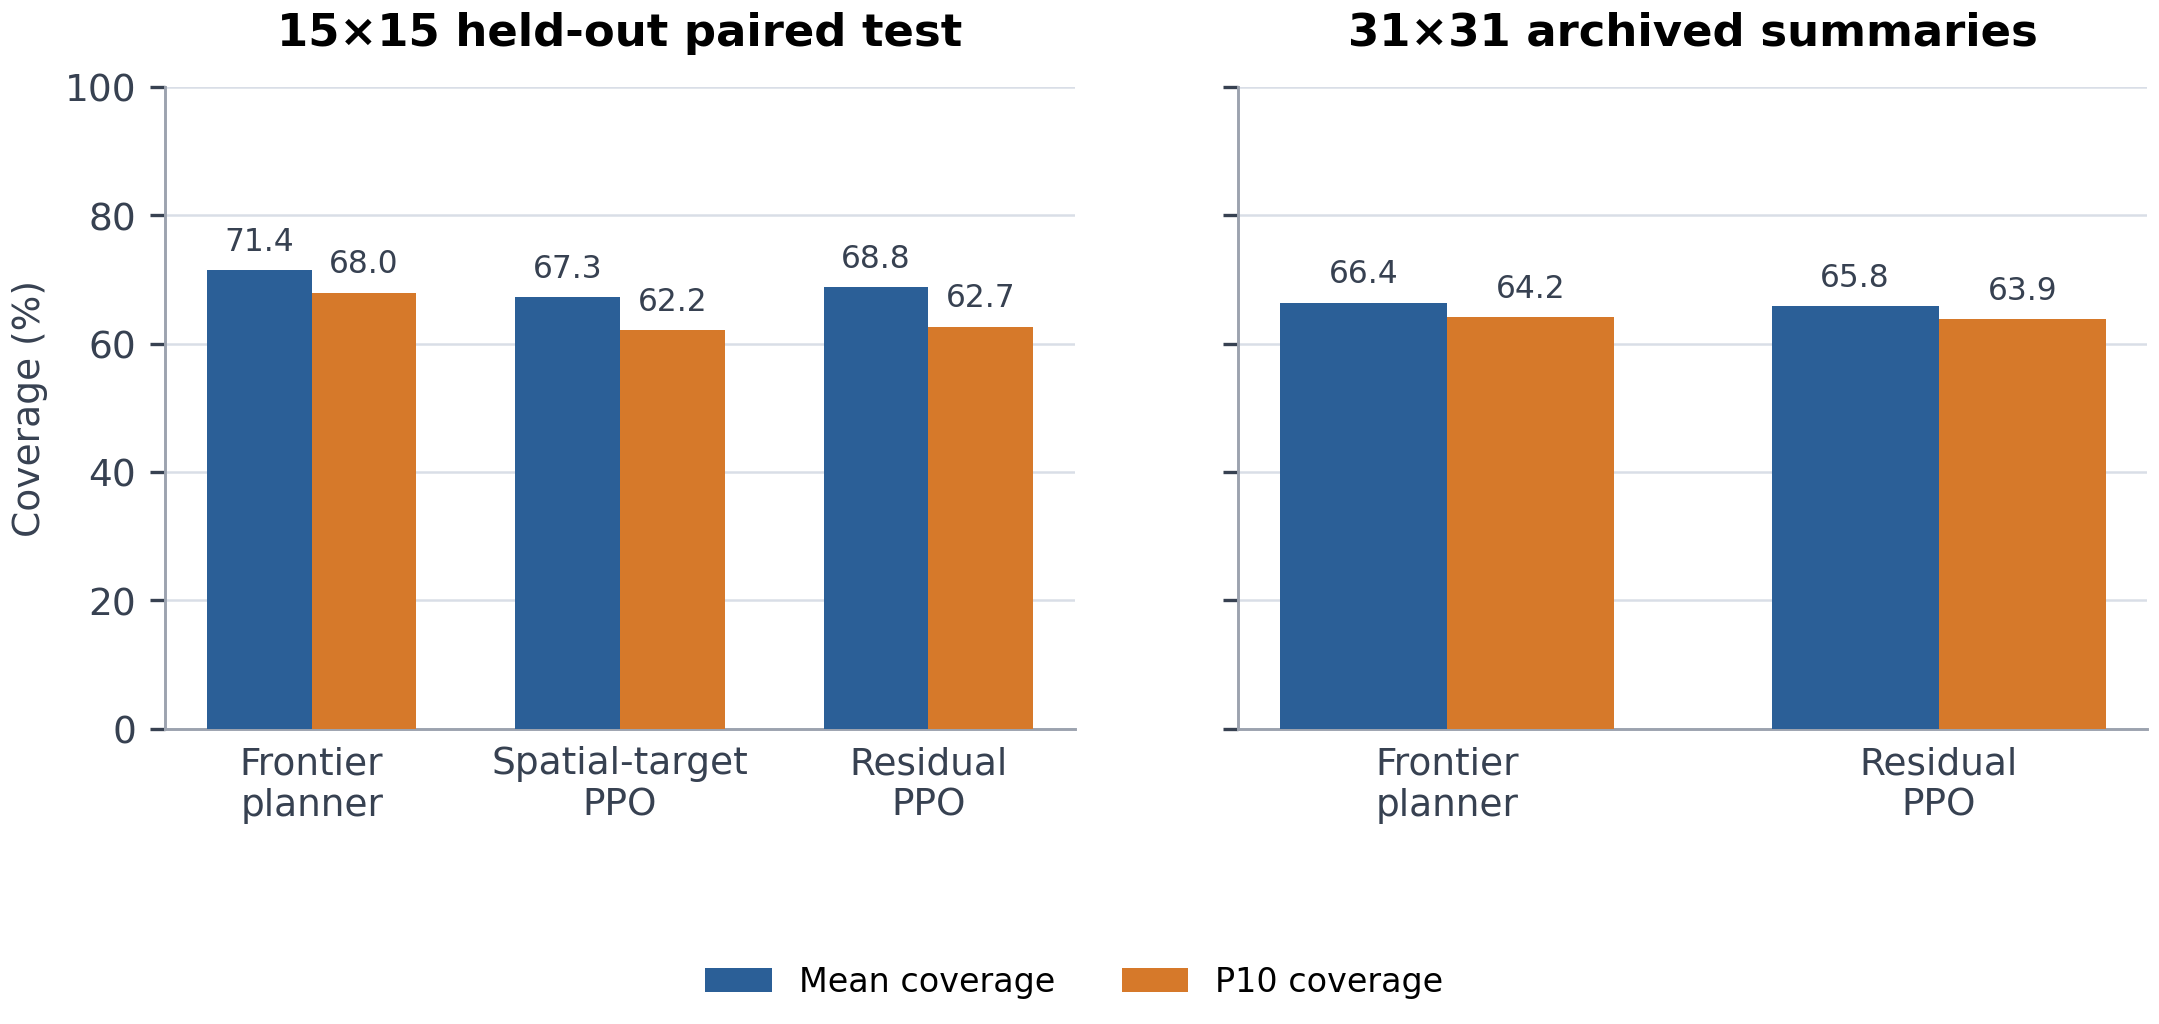
\includegraphics[width=\linewidth]{images/final_benchmark_coverage.png}
\caption{Final 50-episode coverage summaries at both evaluated map sizes. The 15x15 panel is a held-out, map-matched test of the unchanged planner and two selected PPO checkpoints. The 31x31 panel is an archived single-seed, non-paired summary and is descriptive only.}
\label{fig:coverage-comparison}
\end{figure}

The held-out paired-difference distributions are retained in Appendix~\ref{app:supplementary-figures} (Figure~\ref{fig:paired-learned}). They visualise map variation for the two fixed checkpoints without implying training-seed replication.

The held-out planner averages 8.86 repeated forward moves per episode, compared with 9.68 for spatial-target PPO and 8.40 for planner-residual PPO. Their unique-forward ratios are 94.76\%, 93.99\%, and 94.90\%, respectively. The planner's coverage advantage therefore does not arise from an obvious excess of repeated forward movement. For the separate paired planner--oracle control, the oracle's mean advantage is 6.96 percentage points, with a 20,000-resample bootstrap 95\% confidence interval of [6.02, 7.96] and $p=9.06\times10^{-14}$; its matched-map display is retained in Appendix~\ref{app:supplementary-figures}.

Appendix~\ref{app:supplementary-figures} retains the two single-run checkpoint trajectories (Figure~\ref{fig:ppo-trajectories}) as descriptive context for the selected checkpoints; they do not add training replication.

\subsection{Paired ablation of frontier-planner components}

The new 50-map ablation tests the explanation offered for the planner rather than assuming it. On fresh seeds 65,000--65,049, the full planner records 71.57\% mean coverage and 67.91\% P10. Removing resource-recovery routing lowers mean coverage by 10.41 percentage points (95\% bootstrap confidence interval [--12.89, --7.89]; $p=7.88\times10^{-8}$) and P10 to 48.40\%. Removing route revisit costs lowers mean coverage by 1.48 points ([--2.21, --0.79]; $p=0.0029$) and P10 to 64.80\%; repeated forwards rise from 7.72 to 11.70 per episode. Removing the safe-frontier-forward rule lowers mean coverage by 1.86 points ([--3.23, --0.44]; $p=0.044$). In contrast, removing thermal route cost gives an inconclusive $-0.18$ point difference ([--1.04, 0.75]; $p=0.281$). Thus resource timing and revisit control have direct support in this configuration, whereas this finite test does not establish a separate thermal-cost effect. The paired-effect display and non-comparable historical summaries are retained in Appendix~\ref{app:supplementary-figures} and Appendix~\ref{app:historical}, respectively.

\subsection{Sensitivity to observation and resource shifts}

\begin{table}[H]
\caption{Fixed-condition 15x15 sensitivity tests for the same saved residual checkpoint and unchanged planner. Each row is a distinct 50-map paired range. Neither paired interval excludes zero, so neither test establishes a controller advantage under its stated shift.}
\label{tab:sensitivity}
\centering
\small
\begin{tabularx}{\linewidth}{>{\raggedright\arraybackslash}p{0.18\linewidth}>{\centering\arraybackslash}p{0.14\linewidth}>{\centering\arraybackslash}p{0.14\linewidth}>{\centering\arraybackslash}p{0.11\linewidth}>{\centering\arraybackslash}p{0.13\linewidth}Y}
\toprule
Condition & Planner mean / P10 & Residual mean / P10 & Difference & 95\% CI & Exact sign test \\
\midrule
15\% visual-object dropout & 62.69\% / 53.33\% & 64.99\% / 55.42\% & +2.29 pp & [--0.49, 5.20] & $p=0.0789$; 30--17 wins (3 ties) \\
One restorative resource & 56.04\% / 52.84\% & 55.30\% / 53.24\% & -0.74 pp & [--1.64, 0.13] & $p=0.0789$; 17--30 wins (3 ties) \\
\bottomrule
\end{tabularx}
\end{table}

Both intervals in Table~\ref{tab:sensitivity} include zero. This narrow screen therefore establishes neither robustness nor a ranking reversal; Figure~\ref{fig:robustness} retains its matched distributions and exact sign-test outcomes. The separate 31x31, non-paired archive retains the same numerical ordering (planner 66.39\% mean / 64.20\% P10; best residual PPO 65.82\% / 63.89\% P10) in Appendix~\ref{app:historical}; it is descriptive rather than an inferential scaling result.

\section{Discussion}

On the held-out paired 15x15 evaluation, neither selected learned checkpoint
exceeds the frontier planner in either reported coverage measure, and both
mean paired differences have bootstrap intervals below zero. This is an
inferential statement across the 50 fresh maps for these fixed saved models.
The two additional condition shifts have intervals that include zero, and the
31x31 ordering remains descriptive because its learned and planner summaries
are not paired per map. None of these results establishes robustness across
training seeds. The comparison is most useful when read
with the decision structure of each controller. The project does not merely
contrast a neural network with a hand-coded rule. It progressively changes
\emph{where} learning is permitted to make a decision: at every atomic
movement, at a map target, or as a bounded correction to an existing target
score. The following interpretation separates what the measurements support
from conclusions that require controlled ablations.

\subsection{Learning across decision granularities}

The direct-action DQN, PPO/RND, and R2D2 families face the most demanding
decision problem. At every time step they must select \textit{forward},
\textit{left}, or \textit{right}, while also learning the consequences of
heading, revisits, hazards, thermal cost, and resource collection. The reward
for choosing a useful turn may only be realised after many subsequent actions.
Recurrence, replay, intrinsic novelty, and shaped rewards were intended to
address this temporal-credit and exploration problem, but they leave the
policy responsible for both strategic exploration and low-level route
execution.

The planner-assisted policies move learning to a higher-level decision. In the
15x15 configuration, a spatial target is represented in a 29x29 agent-centred
frame, and only safe unvisited cells are legal target choices. After a target
is selected, the deterministic route module returns the next heading-aware
action; the system observes again and replans. The learned target policy
therefore has a more semantically meaningful action than a raw turn, while
the planner enforces local route feasibility. This is a reasonable design for
robotics-inspired exploration because it separates ``where to go'' from ``how
to move there.''

The residual model narrows the learned role further. It retains normalised
planner frontier scores in the target logits at training and evaluation, adds a
small deterministic tie preference, and learns only a bounded spatial
residual. Its performance should consequently not be read as evidence that a
standalone PPO policy learned to solve the environment. Instead, it evaluates
whether a data-driven correction can identify planner mistakes without
damaging the default behaviour. This is the most relevant learned condition
for the project's practical question because it gives learning the strongest
available prior rather than asking it to rediscover safe navigation.

\begin{table}[H]
\caption{Decision granularity in the final comparison. Historical direct-action families are intentionally not assigned a final shared-boundary score.}
\label{tab:granularity}
\centering
\small
\begin{tabularx}{\linewidth}{p{0.25\linewidth}p{0.25\linewidth}Y}
\toprule
Controller class & Learned decision & Deterministic structure retained \\
\midrule
Direct-action DQN, PPO/RND, R2D2 & Atomic action at each step & None beyond input features and reward design \\
Spatial-target PPO & Safe map target & Planner executes each local route action \\
Planner-residual target PPO & Bounded correction to target score & Persistent planner scores and planner route execution \\
Frontier planner & None & Frontier scoring, resource logic, and heading-aware Dijkstra execution \\
\bottomrule
\end{tabularx}
\end{table}

Table~\ref{tab:granularity} makes the contrast in decision structure explicit.
Training objectives, architectures, and data budgets differ across the learned
conditions, so no component-level attribution is justified for their relative
performance. The completed deterministic ablation does, however, hold map
instances fixed while removing individual planner mechanisms. On 50 further
matched maps, zeroing the residual checkpoint's persistent planner scores only
at inference lowers mean coverage by 1.13 points, but the 95\% interval
[--0.41, 2.68] includes zero ($p=0.392$; Figure~\ref{fig:prior-ablation}).
This is therefore not evidence of a resolved inference-time dependence, and
because the checkpoint was trained with the prior, it is not a trained
no-prior ablation. The deterministic reference nevertheless has higher mean
and P10 values than both selected checkpoints.

\subsection{Mean and lower-tail performance}

The result is not only a mean-coverage ordering. At 15x15, the residual policy
reduces the learned mean deficit relative to spatial-target PPO, but it does
not remove it: its paired mean difference is $-2.61$ percentage points. Its
P10 deficit is 5.29 points, larger than its mean deficit. For a safety-aware
exploration task, a learned correction that does not improve the
low-performance tail has not improved the deployable controller under the
stated reliability criterion.

At 31x31 the residual policy is close to the planner, but the non-paired,
single-seed ordering remains descriptive. The two fixed-condition tests add a
further qualification: the residual is directionally higher under detection
dropout and lower under resource scarcity, yet both mean-difference intervals
include zero ($p=0.0789$). They establish neither a learned robustness benefit
nor a universal nominal-planner advantage; the fixed checkpoint is sensitive
to these limited task-distribution changes with unresolved uncertainty.

\subsection{Experimental chronology and implications for model selection}

The final result was reached through parallel investigation, not by replacing
one exhausted branch with another. The learned branch explored off-policy
action values (DQN), on-policy policy gradients (PPO/RND), recurrent
distributional replay (R2D2), and learned target rankers. These selections
cover complementary exploration and memory mechanisms: value-based learning,
policy optimisation, intrinsic novelty, recurrent state, distributional
returns, and imitation or expert guidance. The deterministic branch began
with a simple sweep, then added a belief map and phase structure, before
arriving at frontier planning with thermal, resource, revisit, and heading
costs.

When the final planner became the reference, the research question changed in
a productive way. Rather than continuing to search for a larger unstructured
network, the two final models tested whether learning could improve the
planner's strategic target choice. The first removes the teacher after a
curriculum; the second preserves the planner as a prior. Neither selected
checkpoint exceeds the planner on the held-out paired set. This motivates, but
does not prove, the hypothesis that the hand-designed frontier score already
encodes the dominant useful affordances on these maps.

For future model selection, the findings favour a modular hypothesis over an
end-to-end replacement hypothesis. Keep explicit planning for map update,
local safety, and route execution, and learn only components that are difficult
to specify in advance: uncertainty calibration, value of information, changing
object dynamics, richer sensor noise, or transfer to new layouts. Such a hybrid can
be evaluated fairly by comparing it with an unchanged planner over paired map
seeds, by reporting both gains and regressions, and by treating the planner as
a strong baseline rather than an implementation detail.

\subsection{Task structure, affordances, and oracle performance}

\subsubsection{Structural advantages of the frontier planner}

The result is understandable from the structure of the task. The planner encodes several decisions that the learned models would otherwise have to infer from finite data: which cells are safe, when revisiting is costly, how heading changes route cost, why temperature matters, and when food should override generic coverage. The paired ablation provides direct support for two of these mechanisms in this implementation: removing resource recovery causes a large coverage loss, while removing route revisit costs increases repeated forwards and lowers coverage. It does not isolate a thermal-cost benefit on these 50 maps, so that mechanism should be treated as plausible design structure rather than a demonstrated causal driver. These mechanisms align closely with the evaluation metric. They also remove a large portion of the action-search problem by turning a partially observed local control task into deterministic shortest-path computation over an accumulated map. Certainty-grid and map-based reasoning are long-standing practical tools for this reason \citep{moravec1988certainty}.

The learned hybrids show that a neural component can operate in the structured target-selection representation. Both variants inherit a powerful planner executor, and the residual model also inherits the strategic prior. The completed optimisation procedure did not find target-selection outcomes that outweighed the planner's task-aligned decisions on the held-out maps. The planner therefore retains the higher measured coverage for this project, conditional on the two saved checkpoints.

The result also has an ``affordance'' interpretation. In this environment, a fire or glass cell affords avoidance; meat affords a health-recovery detour; a locally unknown boundary affords information gain. The deterministic planner exposes these affordances directly in a structured map and objective. The learned methods receive the same underlying sensory content but must infer how to trade these effects from reward. Within this Gridworld, the outcome is consistent with the value of explicit affordance-like state and action structure in a data-limited, safety-constrained exploration task. It does not model physical perception or embodiment, so the conclusion should not be transferred uncritically to real robots.

\subsubsection{Implications for autonomous robotic inspection and search}

For a mobile inspection or search robot in an unfamiliar warehouse, industrial site, or damaged indoor area, the task is to turn a partial local map into informative motion without wasting its safety and operating margin on revisits. This architectural separation is consistent with embodied systems that combine learned representation or target selection with explicit spatial reasoning \citep{chaplot2020activeslam,chaplot2020topological,ramakrishnan2020occupancy}. Coverage proxies accessible space and P10 asks whether access remains dependable on difficult maps. Within this abstraction, the result favours explicit spatial memory, cost-aware frontier scoring, and route planning as the decision backbone; learning is a candidate for uncertainty, semantic value, or changing costs rather than a demonstrated replacement.

In deployment, the 5x5 patch would come from local sensor fusion and localisation and the reconstructed map from occupancy or traversability estimation. Health, energy, thermal, and hazard variables abstract safety, battery, environmental burden, and collision risk. The study does not validate hardware: perception, localisation, collision avoidance, safety assurance, representative-site trials, and cross-scene evaluation such as that supported by Habitat remain necessary \citep{brunke2022safe,savva2019habitat,dulacarnold2019challenges}.

\subsection{Limitations and threats to validity}

Several limitations constrain the conclusion.

\begin{enumerate}
    \item \textbf{Training replication and selection.} Each PPO result is one trajectory. The held-out map set was not used for checkpoint selection, but independent learning seeds and a pre-specified validation/test split are needed for a training-procedure claim.
    \item \textbf{Hybrid attribution.} Both final learned methods use the planner for local routing; residual PPO also keeps its target scores. They test whether learning adds value to a planner, not standalone learning.
    \item \textbf{Ablation scope.} The completed ablation removes one deterministic component at a time on 15x15 maps. It does not test interactions among components, learned-policy ablations, alternative parameter values, or enlarged-map mechanisms.
    \item \textbf{Historical and scaling evidence.} Earlier direct-action runs use varying rewards and routines, and the 31x31 preset scales resources with area. Neither is a homogeneous leaderboard or fixed-resource scaling law.
    \item \textbf{Simulation and shift scope.} Object-detection dropout and a resource-count shift are completed only as fixed, stylised 15x15 tests of one saved residual checkpoint. Localisation drift, correlated or semantic perception errors, actuation error, dynamics, safety assurance, and sim-to-real transfer remain untested.
\end{enumerate}

The held-out nominal 15x15 evidence places the planner ahead of both selected learned checkpoints in mean and tail coverage; the two sensitivity tests are inconclusive and 31x31 shows the same ordering descriptively.

\section{Conclusion}

On 50 held-out paired 15x15 maps, the frontier planner achieves 71.41\% mean coverage and 67.96\% P10, above spatial-target PPO (67.32\%, 62.18\%) and residual PPO (68.80\%, 62.67\%); both learned-minus-planner intervals exclude zero. Resource-recovery and revisit ablations support the planner's mechanisms, while the two shift tests are inconclusive. This conclusion is limited to the saved checkpoints and nominal maps: the 31x31 archive is descriptive and one learning seed cannot establish a training-procedure ranking.

\clearpage
\bibliographystyle{tmlr}
\bibliography{references}

\clearpage
\appendix
\section*{Appendices}

\section{Complete archived controller catalogue}
\label{app:catalogue}

Table~\ref{tab:archive} records the complete approach catalogue preserved in the final repository. Names are descriptive translations of historical serial versions. The source code, configuration files, training logs, and any available evaluations remain under \texttt{models/}, \texttt{runs/}, and \texttt{results/}; this table is a reading guide, not a reimplementation claim.

\begin{table}[H]
\caption{Archived learned approaches and their distinguishing mechanism.}
\label{tab:archive}
\centering
\small
\begin{tabularx}{\linewidth}{p{0.31\linewidth}Y}
\toprule
Descriptive final name & Distinguishing mechanism \\
\midrule
Recurrent patch-fusion initial-heuristics DQN & Double DQN with recurrent sensory fusion and structured exploration \\
Windowed coverage DQN & Coverage-window shaping and prioritised recurrent replay \\
Novelty elite-replay DQN & Episodic novelty, elite replay, and self-imitation \\
Future-coverage-credit DQN & Credit for setup actions that lead to later coverage \\
Safe-route-memory DQN & Route-score alignment, thermal exclusion, and memory \\
Goal-conditioned memory DQN & Explicit agent map, goals, and teacher guidance \\
Recurrent PPO/RND frontier prior & Recurrent PPO with RND and a frontier action prior \\
Symmetric recurrent PPO/RND & Symmetry-oriented refinement of the PPO/RND policy \\
Recurrent distributional DQN & Long short-term memory (LSTM), C51 categorical values, duelling Double DQN, prioritised sequences \\
Future-coverage distributional DQN & R2D2-style tuning with adaptive exploration \\
Learned frontier and exploration scorers & Target ranking over a belief-map planner, with ensemble fallback \\
Spatial-target PPO with planner executor & Learned target policy; planner determines each local route action \\
Planner-residual target PPO & Bounded learned target residual over persistent planner scores \\
\bottomrule
\end{tabularx}
\end{table}

\section{Selected archived development results}
\label{app:historical}

The deterministic sweep and two-phase planner record 56.98\% and 60.83\% mean coverage, respectively, in archived 100-episode evaluations. The recurrent patch-fusion DQN reference records 52.53\% final training-time evaluation coverage. The goal-conditioned DQN records 39.18\% final evaluation coverage and 40.58\% holdout coverage. These runs use differing reward functions, evaluation cadences, or environment revisions and are therefore descriptive rather than a joint leaderboard. The archived DQN, PPO/RND, R2D2, and learned-ranker artifacts retain model configurations, training curves, ensemble disagreement, and failure analyses.

\begin{table}[H]
\caption{Selected historical results. These conditions differ from the final shared-boundary comparison and are not jointly ranked.}
\label{tab:historical}
\centering
\small
\begin{tabularx}{\linewidth}{>{\raggedright\arraybackslash}p{0.33\linewidth}>{\raggedright\arraybackslash}p{0.20\linewidth}>{\raggedright\arraybackslash}p{0.17\linewidth}Y}
\toprule
Method / artifact & Reported episodes & Coverage & Interpretation \\
\midrule
Deterministic sweep baseline & 100 & 56.98\% mean & Simple lower baseline \\
Two-phase belief-map planner & 100 & 60.83\% mean & Intermediate planner \\
Recurrent patch-fusion DQN reference & Training evaluation & 52.53\% final eval & Lower learned benchmark \\
Goal-conditioned memory DQN & Training / holdout & 39.18\% / 40.58\% & Later direct-action DQN run \\
Final frontier planner & 50 held-out paired episodes & 71.41\% mean & Shared-observation deterministic reference \\
\bottomrule
\end{tabularx}
\end{table}

\begin{table}[H]
\caption{Archived enlarged-map results. These 31x31 single-seed summaries are not paired per map and are retained for descriptive context only.}
\label{tab:scaling}
\centering
\small
\begin{tabular}{llrrr}
\toprule
Grid & Controller & Episodes & Mean $\cov$ & P10 $\cov$ \\
\midrule
31x31 & Frontier planner & 50 & \textbf{66.39\%} & \textbf{64.20\%} \\
31x31 & Best learned residual PPO (ep. 1,900) & 50 & 65.82\% & 63.89\% \\
31x31 & Final learned residual PPO & 50 & 65.66\% & 64.10\% \\
\bottomrule
\end{tabular}
\end{table}

\section{Supplementary diagnostic figures}
\label{app:supplementary-figures}

The following figures preserve diagnostics and the separate privileged-information control. They are generated by \path{tools/generate_report_figures.py} directly from the curated result archive; the corresponding PNGs are retained under \path{results/figures/}.

\begin{figure}[H]
\centering
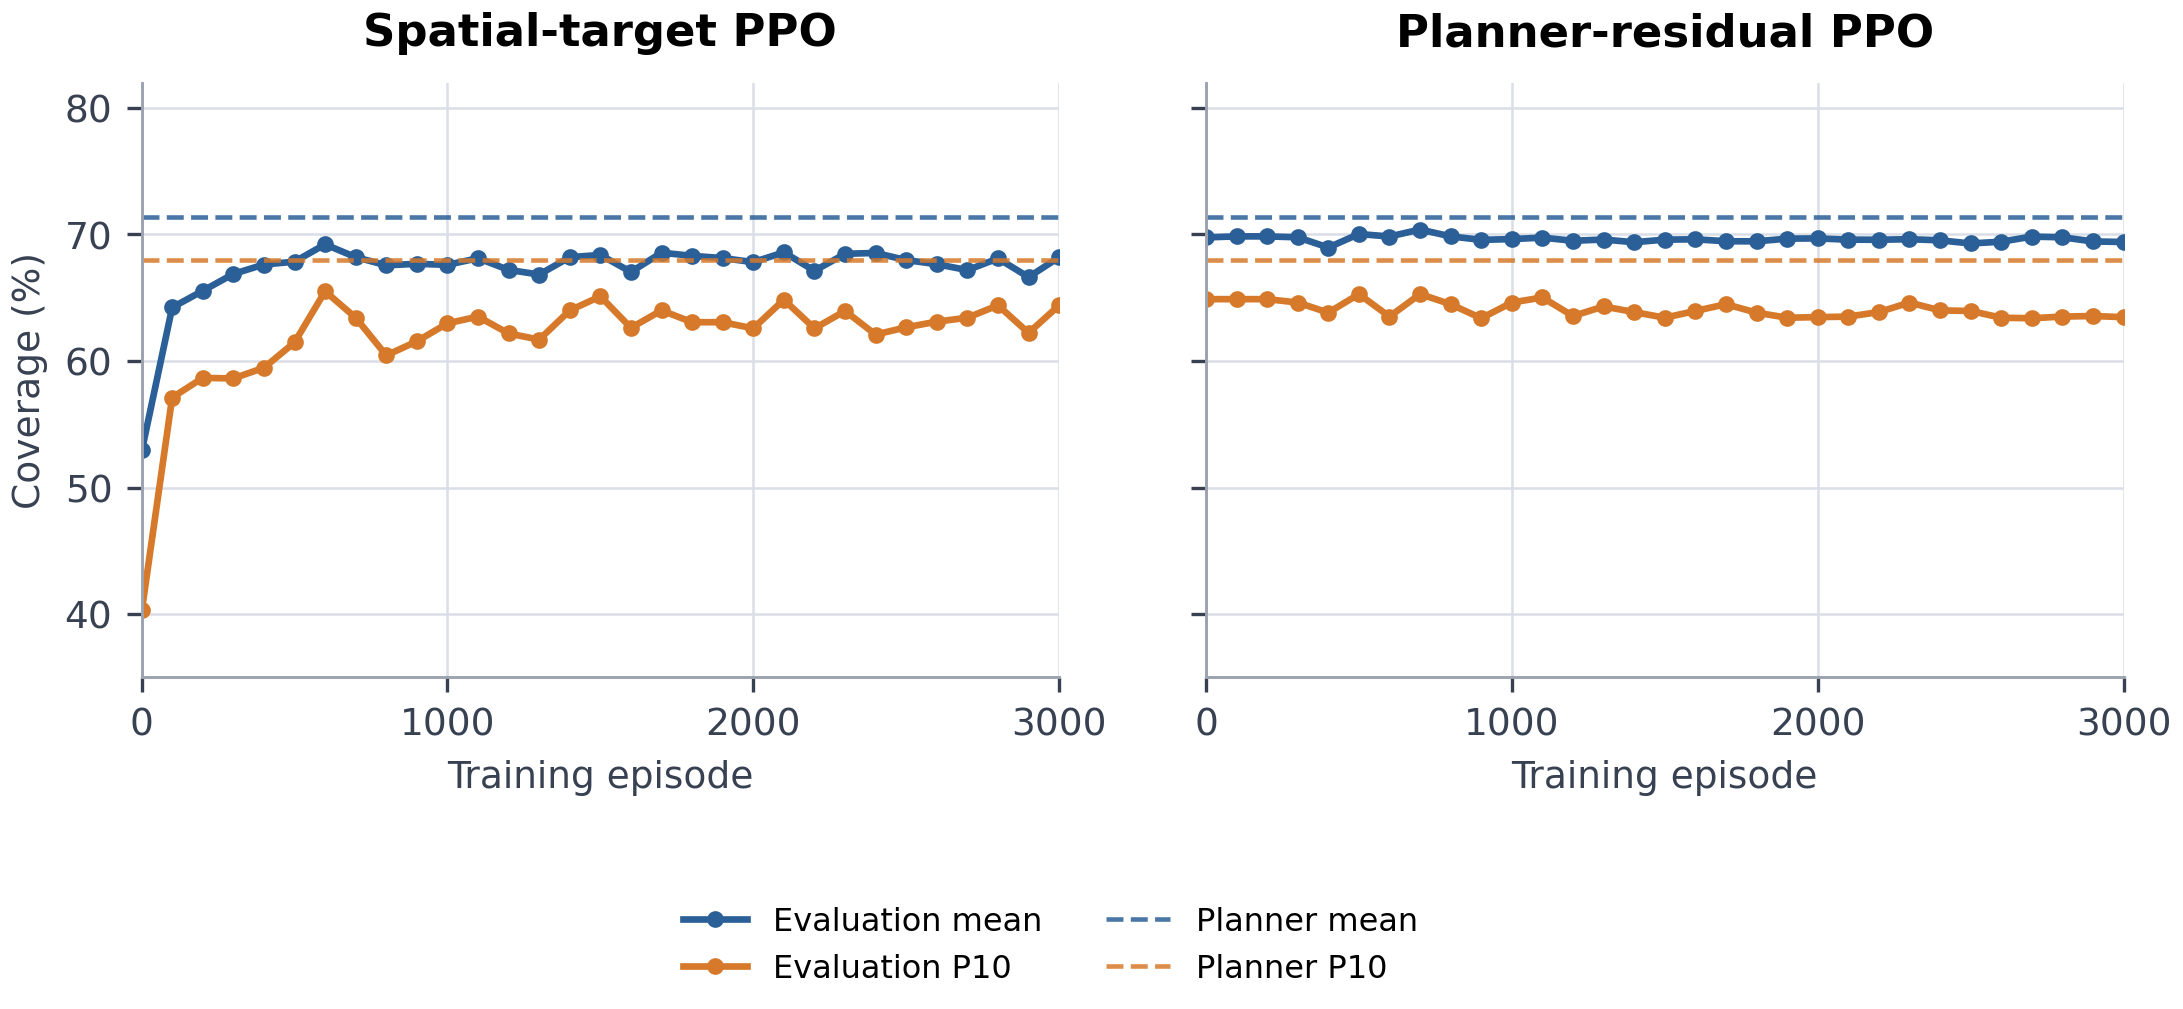
\includegraphics[width=\linewidth]{images/ppo_checkpoint_trajectories.png}
\caption{Periodic 15x15 checkpoint evaluations for the two final learned systems. Solid lines are 50-episode evaluation summaries from one training trajectory; dashed lines are the final 50-map frontier-planner reference. These curves are descriptive diagnostics, not multi-seed confidence estimates or paired comparisons.}
\label{fig:ppo-trajectories}
\end{figure}

\begin{figure}[H]
\centering
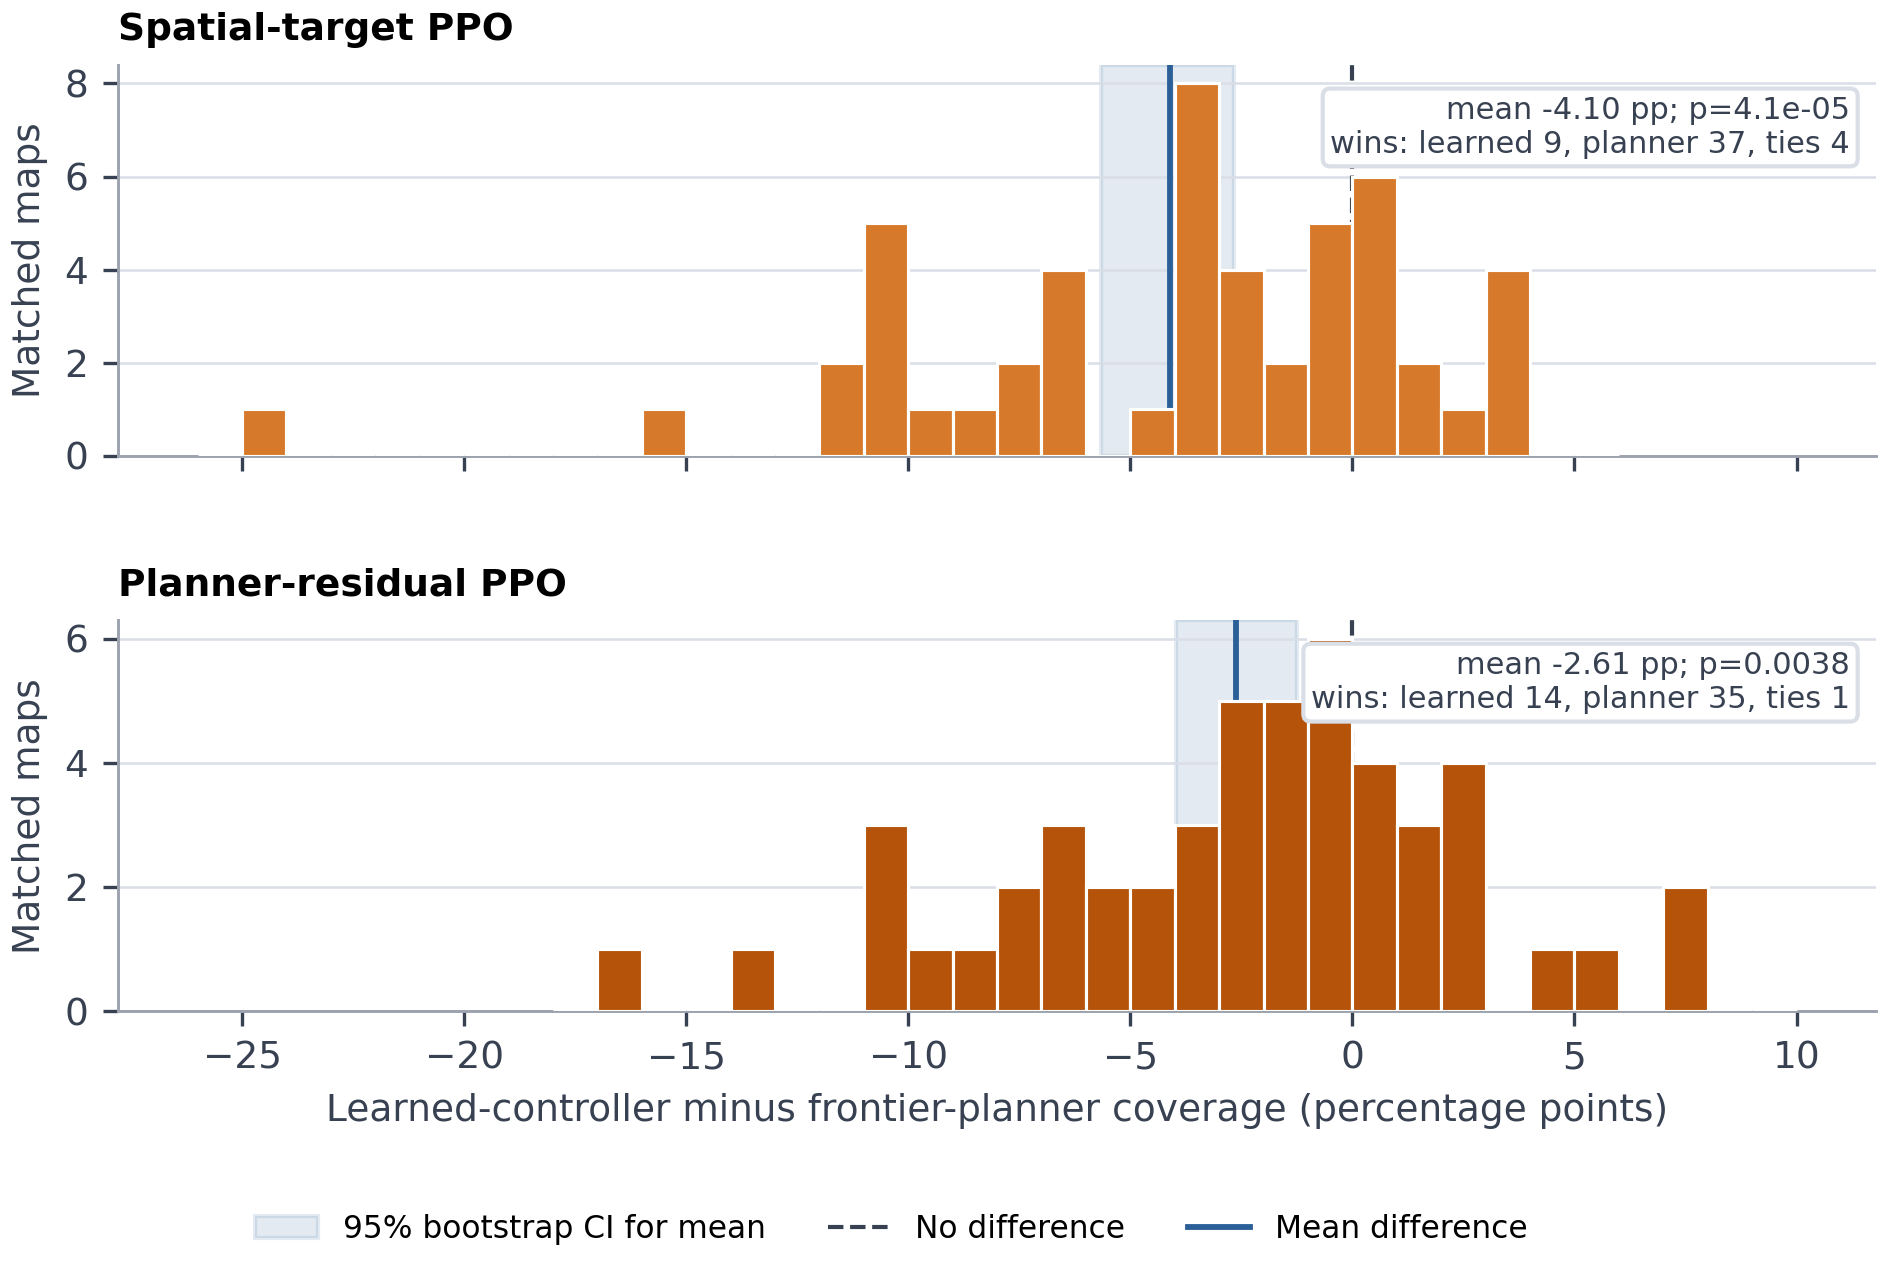
\includegraphics[width=0.82\linewidth]{images/paired_learned_delta_distribution.png}
\caption{Held-out 15x15 paired coverage differences (learned controller minus frontier planner). Shading gives the 20,000-resample bootstrap 95\% confidence interval for the mean; dashed vertical lines mark no difference. Spatial-target PPO has a mean difference of $-4.10$ points and residual PPO $-2.61$ points. These intervals quantify variation across fresh maps for the fixed checkpoints, not training-seed variation.}
\label{fig:paired-learned}
\end{figure}

\begin{figure}[H]
\centering
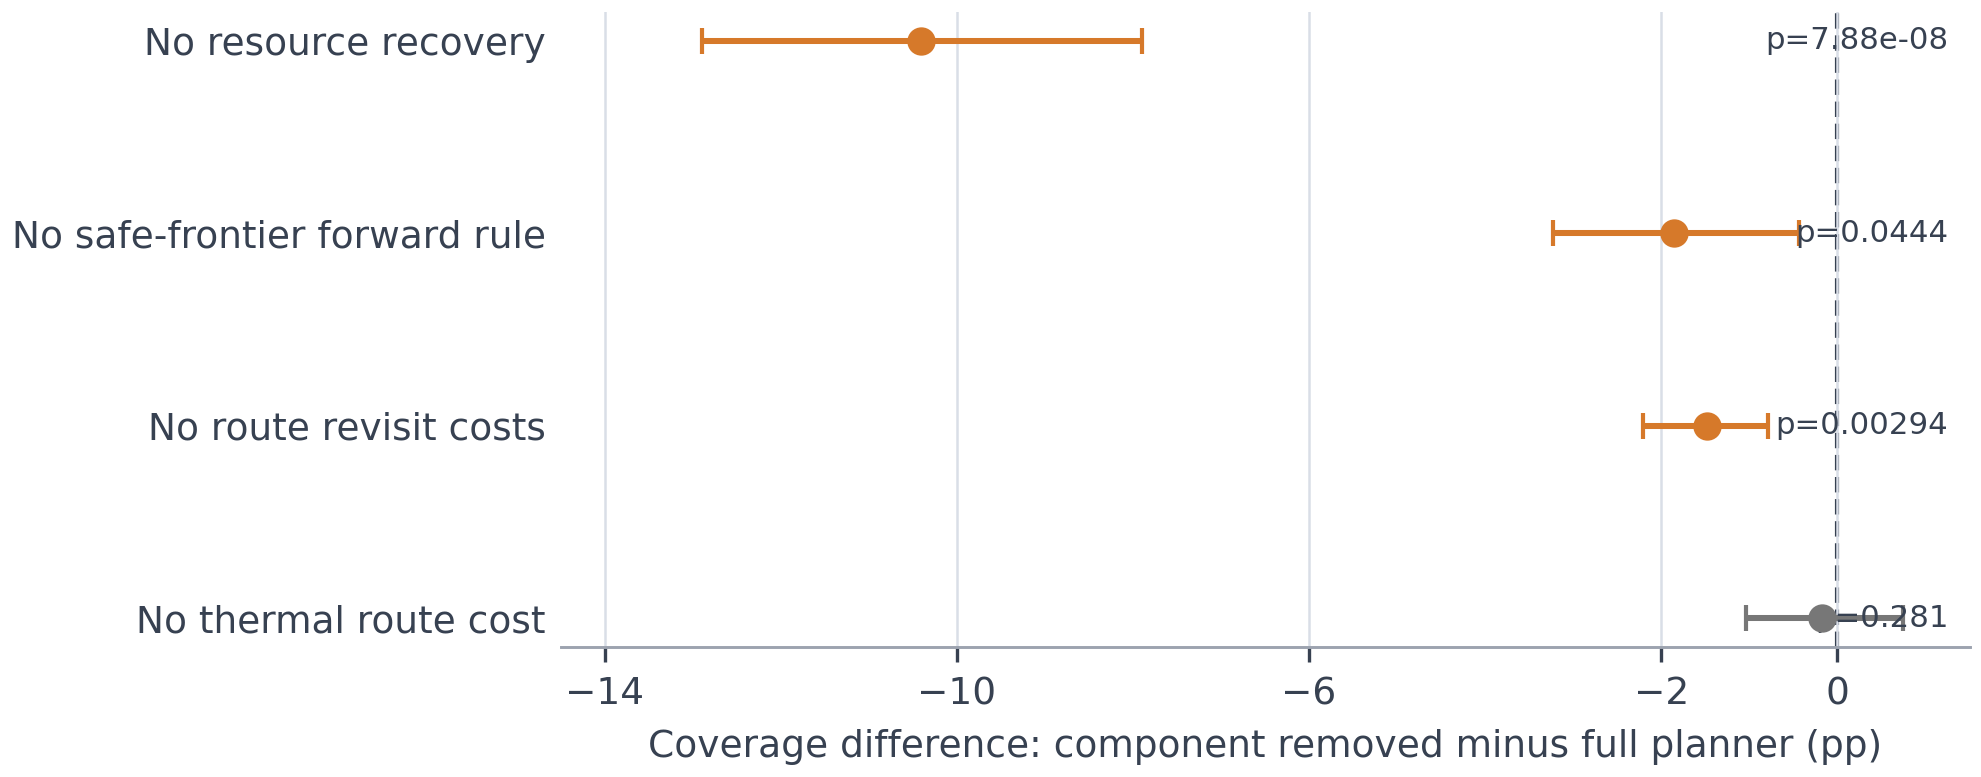
\includegraphics[width=0.92\linewidth]{images/frontier_planner_component_ablation.png}
\caption{Paired 15x15 ablation of the released frontier planner on 50 further held-out maps. Each point is the mean coverage difference after removing one component; bars are 20,000-resample bootstrap 95\% confidence intervals. The thermal-cost interval includes zero, so it is shown as inconclusive rather than as a validated contributor.}
\label{fig:planner-ablation}
\end{figure}

\begin{figure}[H]
\centering
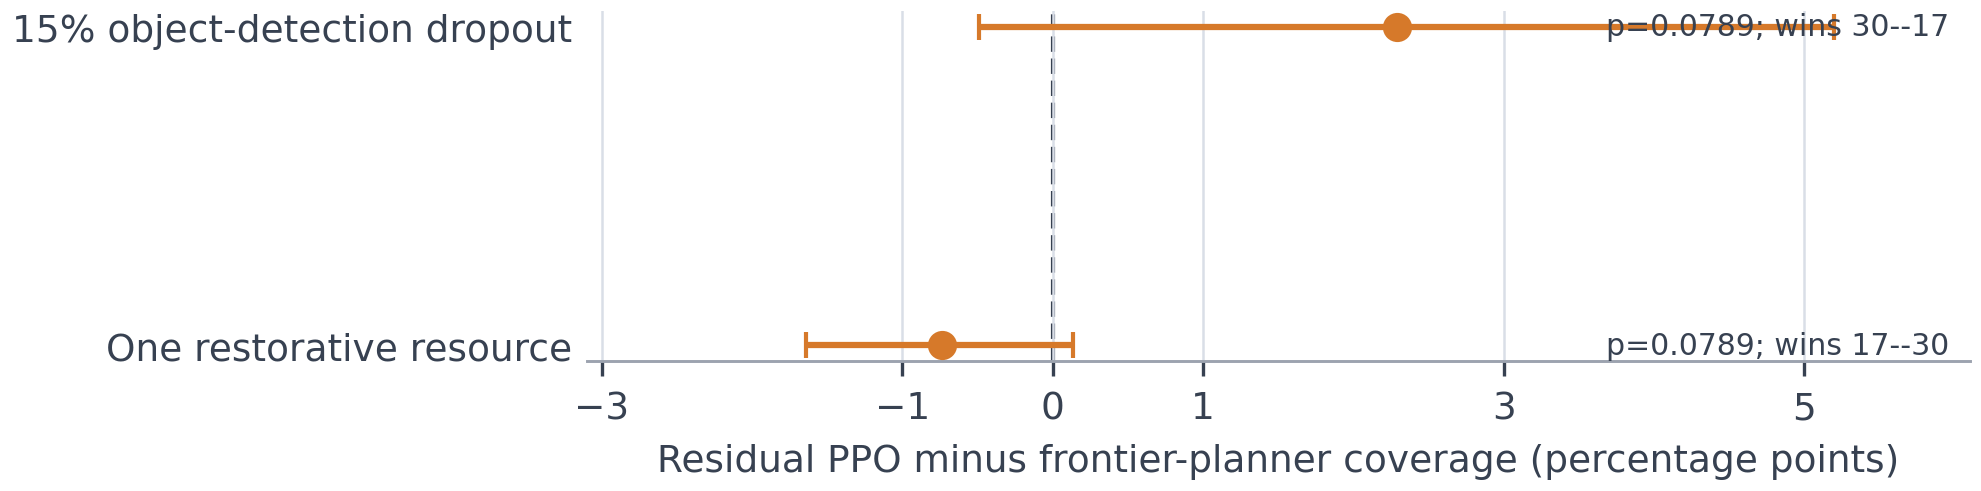
\includegraphics[width=0.92\linewidth]{images/residual_robustness_stress_tests.png}
\caption{Two additional matched 15x15 sensitivity tests of the fixed planner-residual PPO checkpoint. Points show residual PPO minus frontier-planner mean coverage and bars show 20,000-resample bootstrap 95\% intervals across 50 maps. Both intervals include zero. These simple simulated shifts assess neither independent training replication nor real-robot robustness.}
\label{fig:robustness}
\end{figure}

\begin{figure}[H]
\centering
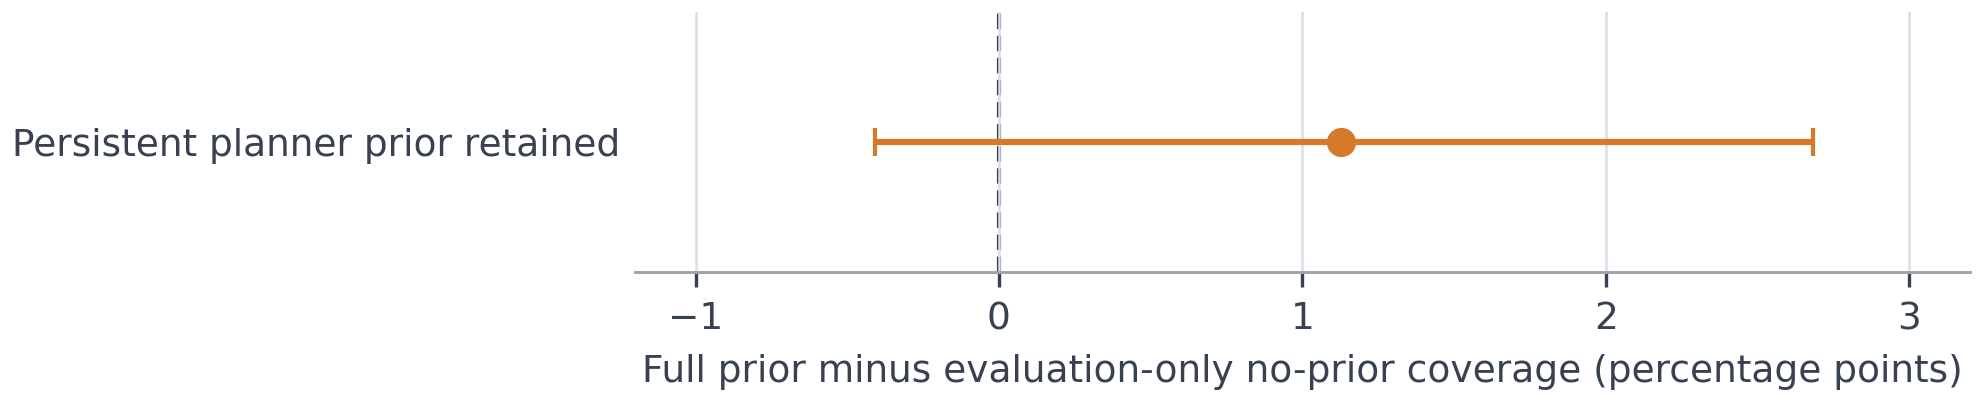
\includegraphics[width=0.90\linewidth]{images/residual_prior_inference_ablation.png}
\caption{Matched evaluation-only persistent-prior diagnostic on 50 further nominal maps. The released residual checkpoint retains the planner target-score weight and tie bonus; the diagnostic zeros both at inference without retraining. The full-prior mean is 1.13 points higher, but its 20,000-resample 95\% interval includes zero. This does not estimate an architecture trained without the prior.}
\label{fig:prior-ablation}
\end{figure}

\begin{figure}[H]
\centering
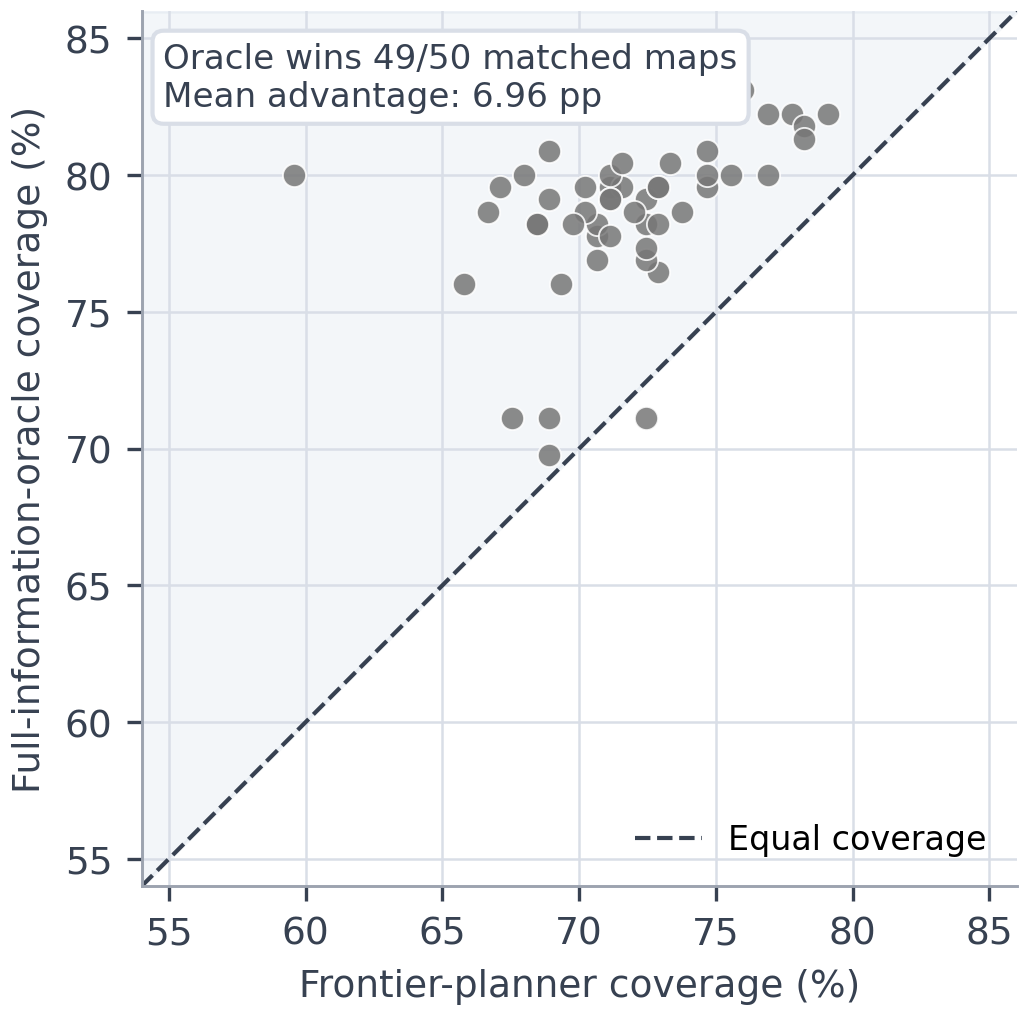
\includegraphics[width=0.60\linewidth]{images/paired_oracle_map_comparison.png}
\caption{Matched 15x15 planner--oracle coverage by map. The full-information oracle wins 49 of 50 shared maps. This visualises the information upper bound only; it is not a learned-versus-planner comparison.}
\label{fig:paired-oracle}
\end{figure}

\begin{figure}[H]
\centering
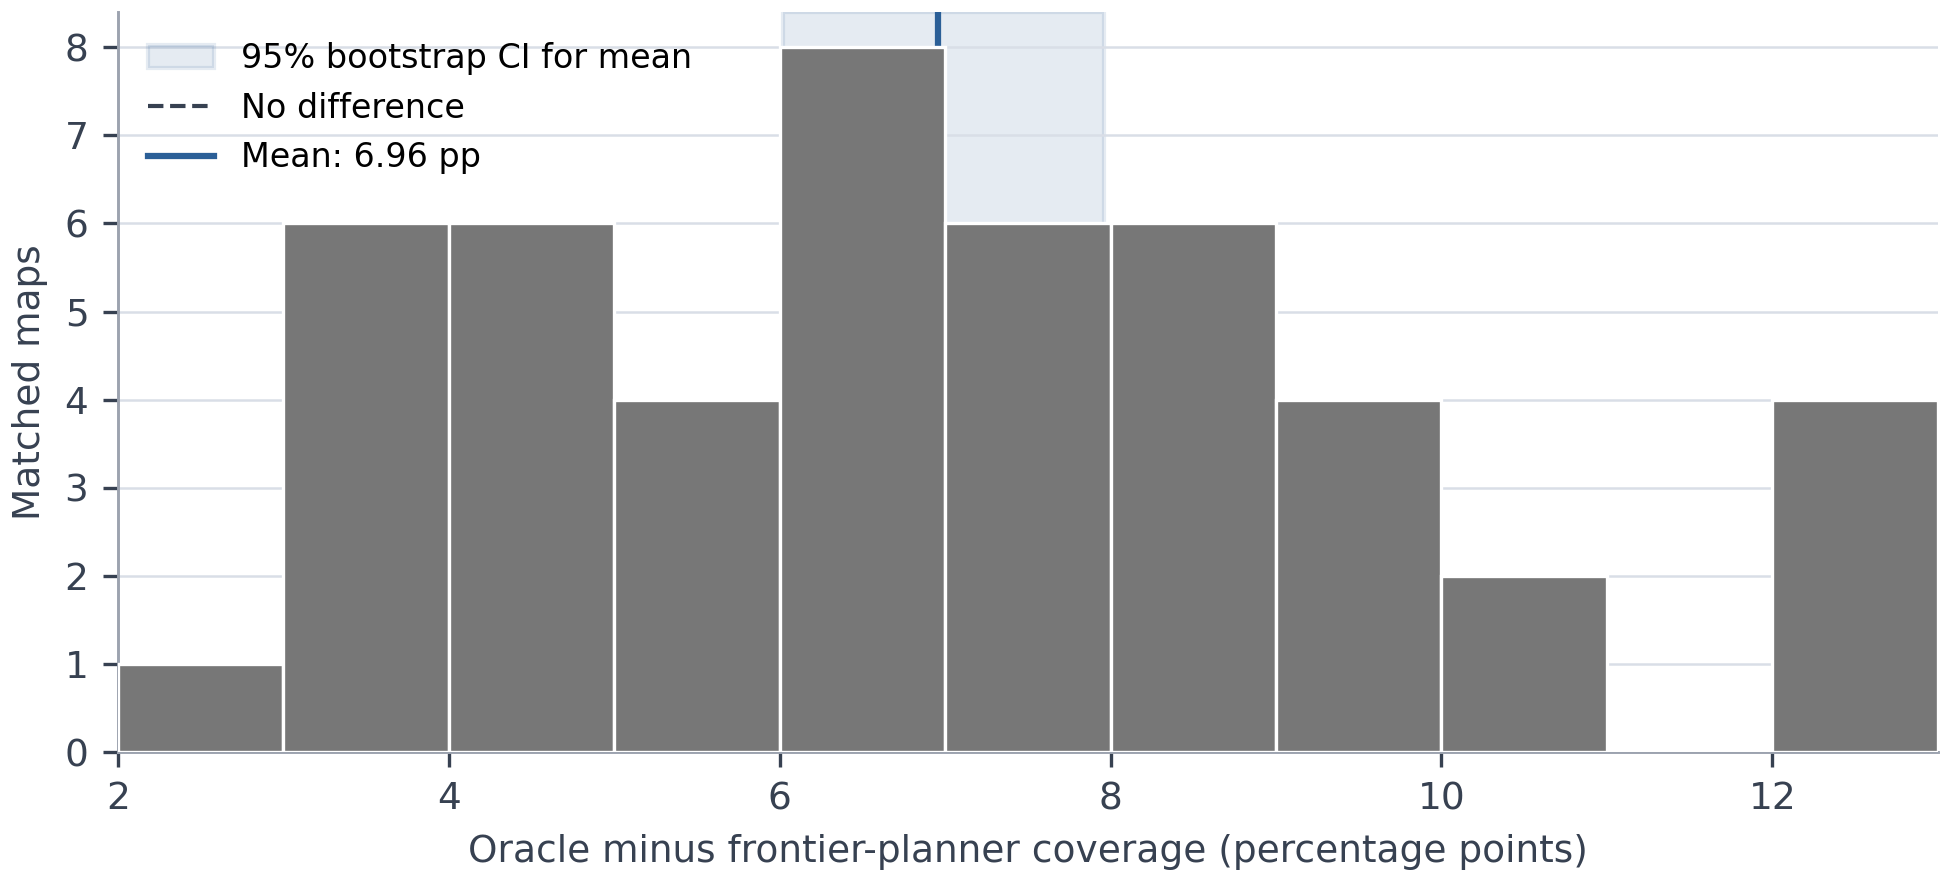
\includegraphics[width=0.93\linewidth]{images/paired_oracle_delta_distribution.png}
\caption{Distribution of the 50 matched full-information-oracle minus frontier-planner coverage differences. The shaded interval is the 20,000-resample bootstrap 95\% confidence interval for the mean paired difference. It quantifies the value of privileged map access, not the effect of learning.}
\label{fig:oracle-delta-distribution}
\end{figure}

\section{Reproducibility and results provenance}
\label{app:provenance}

The final repository separates source, complete raw runs, and a compact result archive. The following exact paths provide the audit trail for the final comparisons:

\begin{itemize}
    \item \path{models/benchmarks/planner_vs_learned/run.py}, \path{results/artifacts/15x15/benchmarks/frontier_planner_vs_learned_heldout/comparison_summary.json}, and \path{results/artifacts/15x15/benchmarks/frontier_planner_vs_learned_heldout/comparison_by_episode.csv} for the held-out paired 15x15 planner--learned test;
    \item \path{models/benchmarks/planner_vs_oracle/run.py}, \path{results/artifacts/15x15/benchmarks/frontier_planner_vs_oracle/comparison_summary.json}, and \path{results/artifacts/15x15/benchmarks/frontier_planner_vs_oracle/comparison_by_episode.csv} for the paired 15x15 control;
    \item \path{models/benchmarks/frontier_planner_component_ablation/run.py}, \path{results/artifacts/15x15/benchmarks/frontier_planner_component_ablation_heldout/comparison_summary.json}, and \path{results/artifacts/15x15/benchmarks/frontier_planner_component_ablation_heldout/comparison_by_episode.csv} for the fresh paired deterministic-component ablation;
    \item \path{models/benchmarks/planner_vs_residual_ppo/run.py}, \path{results/artifacts/15x15/benchmarks/frontier_planner_vs_residual_object_dropout_heldout/comparison_summary.json}, and \path{results/artifacts/15x15/benchmarks/frontier_planner_vs_residual_resource_scarce_heldout/comparison_summary.json} for the two fixed-condition, paired residual sensitivity tests;
    \item \path{tools/analyse_residual_prior_inference_ablation.py}, \path{results/artifacts/15x15/benchmarks/frontier_planner_vs_residual_prior_full_heldout/comparison_by_episode.csv}, \path{results/artifacts/15x15/benchmarks/frontier_planner_vs_residual_without_persistent_prior_heldout/comparison_by_episode.csv}, and \path{results/artifacts/15x15/benchmarks/residual_persistent_prior_inference_ablation_heldout/summary.json} for the matched evaluation-only persistent-prior diagnostic;
    \item \path{results/artifacts/15x15/non_model_based/partial_observation_frontier_planner/baseline_50/planner_config.txt} and \path{results/artifacts/15x15/non_model_based/partial_observation_frontier_planner/baseline_50/summary.json} for the archived 15x15 planner configuration and selection-era summary;
    \item \path{models/model_based/ppo/spatial_target_ppo_with_planner/train.py}, \path{results/artifacts/15x15/model_based/spatial_target_ppo_with_planner/train_config.txt}, and \path{results/artifacts/15x15/model_based/spatial_target_ppo_with_planner/summary.json} for spatial-target PPO;
    \item \path{models/model_based/ppo/planner_residual_target_ppo/train.py}, \path{results/artifacts/15x15/model_based/planner_residual_target_ppo/train_config.txt}, and \path{results/artifacts/15x15/model_based/planner_residual_target_ppo/summary.json} for 15x15 residual PPO;
    \item \path{results/artifacts/31x31/non_model_based/partial_observation_frontier_planner/baseline_50/planner_config.txt}, \path{results/artifacts/31x31/non_model_based/partial_observation_frontier_planner/baseline_50/summary.json}, \path{results/artifacts/31x31/model_based/planner_residual_target_ppo/train_config.txt}, and \path{results/artifacts/31x31/model_based/planner_residual_target_ppo/summary.json} for Table~\ref{tab:scaling}; and
    \item \path{tools/analyse_paired_oracle.py}, which reproduces the oracle-control bootstrap interval and exact sign test reported in Section~\ref{sec:results}; and
    \item \path{tools/generate_report_figures.py}, which reproduces Figures~\ref{fig:coverage-comparison}, \ref{fig:paired-learned}, \ref{fig:planner-ablation}, \ref{fig:robustness}, \ref{fig:prior-ablation}, \ref{fig:paired-oracle}, \ref{fig:ppo-trajectories}, and \ref{fig:oracle-delta-distribution} from the archived metrics.
\end{itemize}

Raw traces and checkpoints are intentionally kept in \texttt{runs/} rather than duplicated in the compact result archive. Legacy artifacts are all classified as 15x15; the final repository preserves their manifests and original run names for auditability.

\section{Recommended evaluation protocol}

The strongest follow-up is not another isolated training run. It is a
pre-specified experiment that gives the planner and learned hybrids the same
opportunity to demonstrate improvement. First, generate and store disjoint
training, validation, and final test seed sets for each map size. The final
test maps should remain unused for reward shaping, checkpoint selection, and
hyperparameter tuning. Second, train multiple independent instances of each
learned method with different learning seeds while keeping the environment
generator, training budget, and observation interface fixed. The deterministic
planner should be evaluated unchanged on the same final test maps.

The reporting unit should be the paired per-map difference in coverage between
a learned controller and the planner. Aggregate mean coverage remains useful,
but paired differences reveal whether an apparent average gain is widespread
or is driven by a small number of maps. Report the mean difference, median
difference, P10 coverage for each controller, the fraction of maps won by each
controller, and a bootstrap confidence interval across maps. Health loss,
repeated forwards, and unique-forward ratio should be retained so that a gain
in coverage cannot conceal inefficient or unsafe motion.

The completed planner ablation should be extended to identify which learned
hybrid components are useful. Compare target PPO with and without planner
route execution, residual PPO with and without persistent planner target
scores, and interactions between deterministic resource routing, thermal cost,
and revisit penalties. These experiments would distinguish the value of a map
representation from the value of a particular frontier score and route
executor. The same matrix should then be evaluated at 15x15 and 31x31 so that
the scaling claim remains a genuine controller comparison.

\begin{table}[H]
\caption{Recommended controlled follow-up. Each row addresses a limitation of the completed project while preserving its useful partial-observation setting.}
\label{tab:followup}
\centering
\small
\begin{tabularx}{\linewidth}{p{0.29\linewidth}Y}
\toprule
Design element & Requirement and purpose \\
\midrule
Independent splits & Freeze validation and held-out test seed sets before model selection \\
Multiple learning seeds & Estimate training variance rather than reporting one trajectory \\
Paired map evaluation & Compare every learned run and planner on identical map fingerprints \\
Safety diagnostics & Report P10, health loss, repeated forwards, and coverage jointly \\
Planner ablations & Isolate target prior, route executor, resource logic, thermal cost, and revisit control \\
Scaling matrix & Train and test all valid controllers at 15x15 and 31x31 \\
\bottomrule
\end{tabularx}
\end{table}

This protocol preserves the project's central insight: the planner is the
baseline that every learned method must surpass. It would establish whether a
learned residual delivers a reliable gain over the explicit, auditable
controller and would identify which task components should remain explicitly
planned.

\section*{Generative AI usage disclosure}
This work follows UCL Category 2 guidance for generative artificial intelligence (GenAI): tools are used in an assistive role for drafting, editing, and code support. All analysis, decisions, and final content are authored and verified by the student.

\end{document}
